
\begin{frame}
   \frametitle{Lazily Evaluated Marginal Utility Roadmaps}
   \begin{tikzpicture}[font=\small]
   \draw[step=1,black!15,very thin,opacity=\gridopacity] (0,0) grid (12,8);
   \tikzset{>=latex} % arrow heads

      \node[fill=blue!5,rounded corners,anchor=north,minimum width=9.5cm,minimum height=6.7cm] (alg) at (6,7.75) {};
      \node[left=0.1cm of alg.north,anchor=north] {\begin{minipage}{9cm}
         \begin{algorithmic}[1]
         \Procedure {LEMUR}{$q_{\ms{start}}, q_{\ms{goal}}, x,
            \mathcal{M}.\grave{p}, \mathcal{M}.\hat{x}, \lambda_p$}
         \State $G \leftarrow$ graph with
            $V = \{ q_{\ms{start}}, q_{\ms{goal}} \}$
            and $E = \emptyset$
         %\State $w_0 : E \rightarrow \mathbb{R}^{+}$ \Comment mutable edge weight function
         \State $w_0(e) = \lambda_p \, \grave{p}(e) + (1\!-\!\lambda_p) \, \hat{x}(e) \quad \forall e \in G.E$
         \For {iteration $i \in 1, 2, \dots$}
            \State $\pi_i = \displaystyle\argmin_{\pi \in \Pi(G)} 
               \mbox{len}\left(\pi, w\right)$
               \Comment incremental search
            \If {$\pi_i$ is {\bf null}}
               \State $V_{\ms{new}}, E_{\ms{new}} \leftarrow$ new densified roadmap batch
               \State $G.V \stackrel{\tiny +}\leftarrow V_{\ms{new}};
                  \;\; G.E \stackrel{\tiny +}\leftarrow E_{\ms{new}}$
               \State $w(e) \leftarrow \lambda_p \, \grave{p}_i(e) + (1\!-\!\lambda_p) \, \hat{x}_i(e)
                  \; \forall \; e \in E_{\ms{new}}$
               \State {\bf continue}
            \EndIf
            \If {$\pi_i$ is fully evaluated}
               \State \Return $\pi_i$
            \EndIf
            \State $e_i \leftarrow$ select unevaluated edge from $\pi_i$
            \State evaluate $e_i$
            \State $\hat{x}(e_i) \leftarrow x(e_i); \;\; \grave{p}(e_i) \leftarrow 0$
               \Comment e.g. evaluate fully
            \State $w_i(e_i) \leftarrow
               \lambda_p \, \grave{p}(e_i) + (1\!-\!\lambda_p) \, \hat{x}(e_i)$
         \EndFor
         \EndProcedure
         \end{algorithmic}
      \end{minipage}};


   \end{tikzpicture}
\end{frame}

\begin{frame}
   \frametitle{Maximizing Utility: HERB Bin Experiments}
   \begin{tikzpicture}[font=\small]
      \tikzset{>=latex} % arrow heads
      \draw[step=1,black!15,very thin,opacity=\gridopacity] (0,0) grid (12,8);

      \node at ( 3.75,6.4) {
         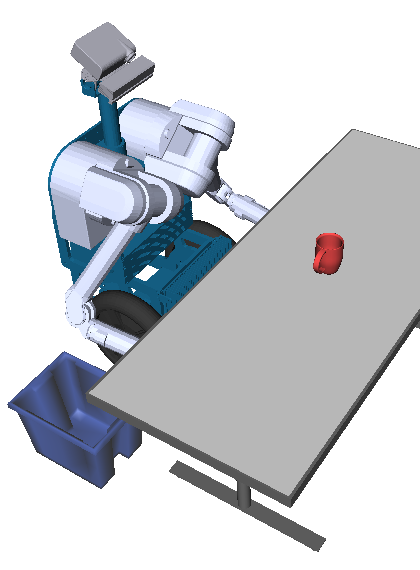
\includegraphics[width=1.7cm]{figs/herbbin/step0cropped.png}
         \;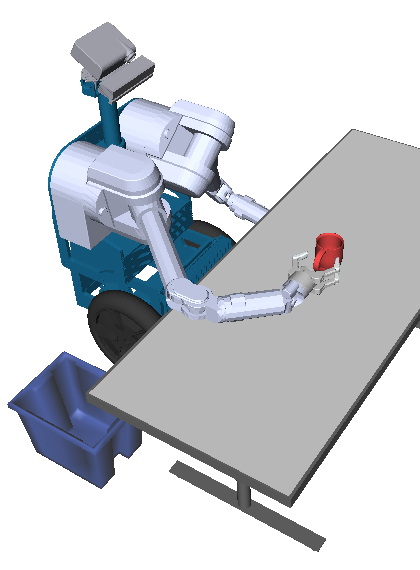
\includegraphics[width=1.7cm]{figs/herbbin/step01cropped.png}};

      %\node[inner sep=0pt] (vidnode) at (9.5,6.5) {%
      %   \href{\tikzvidtarget{incbi-roadne}}{%
      %   \includegraphics[width=4cm]{videos/workcell-cropped.png}}};
      %\tikzvidplayat{incbi-roadne}{vidnode}{videos/workcell-cropped.mp4}{}

      \node at (3.5,2.5) {\includegraphics[width=7cm]{build/lemur-sq/herbbin0}};

      \node at (9.5,2.5) {\includegraphics[height=4cm]{build/multistep-prescribed/herbbinnom-g1ll-lemuronly}};
      
   \end{tikzpicture}
\end{frame}

\begin{frame}
   \frametitle{Maximizing Utility: Workcell Experiments}
   \begin{tikzpicture}[font=\small]
      \tikzset{>=latex} % arrow heads
      \draw[step=1,black!15,very thin,opacity=\gridopacity] (0,0) grid (12,8);

      \node at ( 3.75,6.4) {
         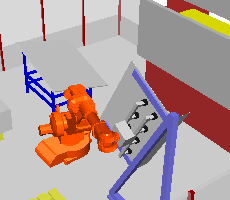
\includegraphics[width=2.7cm]{figs/workcell/cropped-config-f.png}
         \;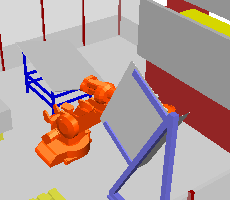
\includegraphics[width=2.7cm]{figs/workcell/cropped-config-g.png}};

      \node[inner sep=0pt] (vidnode) at (9.5,6.5) {%
         \href{\tikzvidtarget{workcell-cropped}}{%
         \includegraphics[width=4cm]{videos/workcell-cropped.png}}};
      \tikzvidplayat{workcell-cropped}{vidnode}{videos/workcell-cropped.mp4}{}

      \node at (3.5,2.5) {\includegraphics[width=7cm]{build/lemur-sq/workcellfg}};

      \node at (9.5,2.5) {\includegraphics[height=4cm]{build/multistep-prescribed/workcell-g1ll-lemuronly}};
      
   \end{tikzpicture}
\end{frame}

